\documentclass[svgnames,11pt]{beamer}
\input{/home/tof/Documents/Cozy/latex-include/preambule_commun.tex}
\input{/home/tof/Documents/Cozy/latex-include/preambule_beamer.tex}
%\usepackage{pgfpages} \setbeameroption{show notes on second screen=left}
\author[]{Christophe Viroulaud}
\title{Traitement de données\\Le Titanic}
\date{\framebox{\textbf{Donn 01}}}
%\logo{}
\institute{Seconde - SNT}


\begin{document}
\begin{frame}
    \titlepage
\end{frame}
\section{Histoire}
\begin{frame}
    \frametitle{Histoire}
    Le RMS Titanic est un paquebot transatlantique britannique qui fait naufrage dans l'océan Atlantique Nord en 1912 à la suite d'une collision avec un iceberg, lors de son voyage inaugural de Southampton à New York.\\ La coque du Titanic était pourvue de seize compartiments étanches servant à protéger le navire en cas de voies d'eau ou d'avaries importantes, ce qui lui donna la réputation de paquebot « insubmersible » et conduit les médias contemporains à le présenter comme l'un des navires les plus sûrs.
    \begin{center}
        \centering
        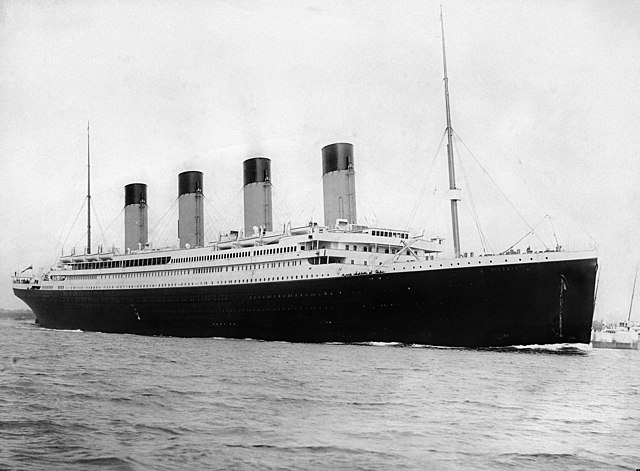
\includegraphics[width=4cm]{ressources/titanic.jpg}
        \captionof{figure}{Le Titanic}
        \label{IMG}
    \end{center}
\end{frame}
\begin{frame}
    \frametitle{}

    Le 14 avril 1912, quatre jours après le commencement de son voyage inaugural, il heurte un iceberg à 23 h 40 (heure locale) et coule le 15 avril 1912 à 2 h 20 au large de Terre-Neuve.\\
    L'épave du Titanic est localisée le 1er septembre 1985 par le professeur Robert Ballard. Elle gît à 3 843 mètres de profondeur à 650 km au sud-est de Terre-Neuve\footnote{Source: \url{https://fr.wikipedia.org/wiki/Titanic}}.

    Les données étudiées par la suite, recensent les informations des passagers du navire.
\end{frame}
\section{Découvrir la structure des données}
\begin{frame}
    \frametitle{Découvrir la structure des données}
    Les données sont contenues dans un fichier \emph{csv (Comma Separated Values)}.
    \begin{activite}
        \begin{enumerate}
            \item Sur le site \url{https://cviroulaud.github.io}, télécharger le dossier compressé \emph{titanic.zip} et en extraire le fichier \textbf{titanic.csv}
            \item Ouvrir le fichier avec \textbf{le bloc-notes de Windows}. Observer le symbole utilisé pour séparer les données.
        \end{enumerate}
    \end{activite}

\end{frame}
\begin{frame}
    \frametitle{}
    \setcounter{compteuractivite}{0}
    \begin{activite}
        \begin{enumerate}
            \setcounter{enumi}{2}
            \item Ouvrir un fichier \textbf{LibreOffice Texte} pour noter les réponses.
            \item Ouvrir le fichier de données à l'aide du logiciel \textbf{LibreOffice Calc}. Le logiciel repère les symboles et classe les données dans des colonnes.
            \item La première ligne présente les \textbf{descripteurs}. Que représentent ces termes?
            \item Pour le descripteur \emph{sexe}, à quoi correspond la valeur \emph{1} ?
            \item Pour le descripteur \emph{tarif}, à quoi correspond la valeur indiquée pour chaque objet ?
        \end{enumerate}
    \end{activite}

\end{frame}
\begin{frame}
    \frametitle{Correction}
\begin{aretenir}[]
Un fichier \textbf{csv (Comma Separated Values)} rassemble des informations sur un thème. Les données sont classées selon des \textbf{descripteurs}. Chaque ligne du fichier représente un \textbf{enregistrement}.
\end{aretenir}
    \begin{itemize}
        \item Un descripteur représente une caractéristique des données contenues dans le fichier.
        \item Le 1 représente les hommes et le 2 les femmes.
        \item Le prix du billet payé par chaque passager est donné dans la colonne \emph{tarif}. Il est donné en Livre Sterling. On peut remarquer que certains passagers n'ont pas payé.
    \end{itemize}

\end{frame}
\section{Exploitation des données}
\begin{frame}
    \frametitle{Exploitation des données}

    Le tableur LibreOffice propose des fonctions de calculs automatiques. Une méthode possible consiste à:
\begin{enumerate}
    \item se placer dans une case vide,
    \item entrer le signe \textbf{\texttt{=}} puis la fonction désirée. Par exemple, \textbf{\texttt{MOYENNE}} (ou \textbf{\texttt{AVERAGE}} en anglais),
    \item entrer la plage de calcul; exemple: \textbf{\texttt{A2:A10}} pour prendre les cellules A2 à A10.
\end{enumerate}

\vspace{1cm}
Exemple:
\begin{center}
    \textbf{\texttt{=MOYENNE(A2:10)}}
\end{center}
\end{frame}
\begin{frame}

    \begin{activite}
        À l’aide des fonctions usuelles du tableur, déterminer:
    \begin{enumerate}
        \item l’âge moyen des passagers,
        \item le tarif moyen payé,
        \item le tarif le plus élevé qui a été payé.
    \end{enumerate}
    \end{activite}

\end{frame}
\begin{frame}
    \frametitle{Avant de regarder la correction}
\begin{center}
    \centering
    \includegraphics[width=3cm]{/home/tof/Documents/Cozy/latex-include/stop.png}
    \end{center}
{\Large
    \begin{itemize}
        \item Prendre le temps de réfléchir,
        \item Analyser les messages d'erreur,
        \item Demander au professeur.
    \end{itemize}
}
\end{frame}
\begin{frame}[fragile]
    \frametitle{Correction}

    \begin{center}
    \begin{lstlisting}[language=Python , basicstyle=\small, xleftmargin=2em, xrightmargin=2em]
= MOYENNE(E2 : E1310)
\end{lstlisting}
    \captionof{code}{Âge moyen}
    \label{age}
    \end{center}
L'âge moyen est 29,90 ans.
\end{frame}
\begin{frame}[fragile]
    \frametitle{Correction}

    \begin{center}
    \begin{lstlisting}[language=Python , basicstyle=\small, xleftmargin=2em, xrightmargin=2em]
= MOYENNE(F2 : F1310)
\end{lstlisting}
    \captionof{code}{Tarif moyen}
    \label{age}
    \end{center}
Le tarif moyen est 33,36£.
\end{frame}
\begin{frame}[fragile]
    \frametitle{Correction}

    \begin{center}
    \begin{lstlisting}[language=Python , basicstyle=\small, xleftmargin=2em, xrightmargin=2em]
= MAX(F2 : F1310)
\end{lstlisting}
    \captionof{code}{Tarif maximum}
    \label{age}
    \end{center}
Le tarif maximum est 512£.
\end{frame}
\section{Filtrer les données}
\begin{frame}
    \frametitle{Flitrer les données}

    L’outil \textbf{Données/Autofiltre} permet de réaliser des filtres sur les valeurs de chaque descripteur.
    \begin{activite}
    \begin{enumerate}
        \item Sélectionner toutes les colonnes des données.
        \item  Activer l'outil \textbf{Données/Autofiltre},
        \item Trier les tarifs par ordre croissant. Construire et compléter le tableau suivant :
        \begin{center}
            \begin{tabular}{|*{5}{c|}}
                \hline
                Tarif payé & $[0;50[$& $[50;100[$& \dots& $[500;550[$\\
                \hline
                Effectif&&&&\\
                \hline
            \end{tabular}
        \end{center}
        \item Dans le tableur, créer une nouvelle feuille, recopier le tableau et construire une représentation graphique correspondante aux données.
    \end{enumerate}
    \end{activite}

\end{frame}
\begin{frame}
    \frametitle{Avant de regarder la correction}
\begin{center}
    \centering
    \includegraphics[width=3cm]{/home/tof/Documents/Cozy/latex-include/stop.png}
    \end{center}
{\Large
    \begin{itemize}
        \item Prendre le temps de réfléchir,
        \item Analyser les messages d'erreur,
        \item Demander au professeur.
    \end{itemize}
}
\end{frame}
\begin{frame}
    \frametitle{Correction}

    \begin{itemize}
        \item $[0;50[ \rightarrow 1063$
        \item $[50;100[ \rightarrow 161$
        \item $[100;150[ \rightarrow 33$
        \item $[150;200[ \rightarrow 13$
        \item $[200;250[ \rightarrow 21$
        \item $[250;300[ \rightarrow 13$
        \item $[300;350[ \rightarrow 0$
        \item $[350;400[ \rightarrow 0$
        \item $[400;450[ \rightarrow 0$
        \item $[450;500[ \rightarrow 0$
        \item $[500;550[ \rightarrow 4$
    \end{itemize}

\end{frame}
\begin{frame}
    \frametitle{Correction}

    \begin{center}
    \centering
    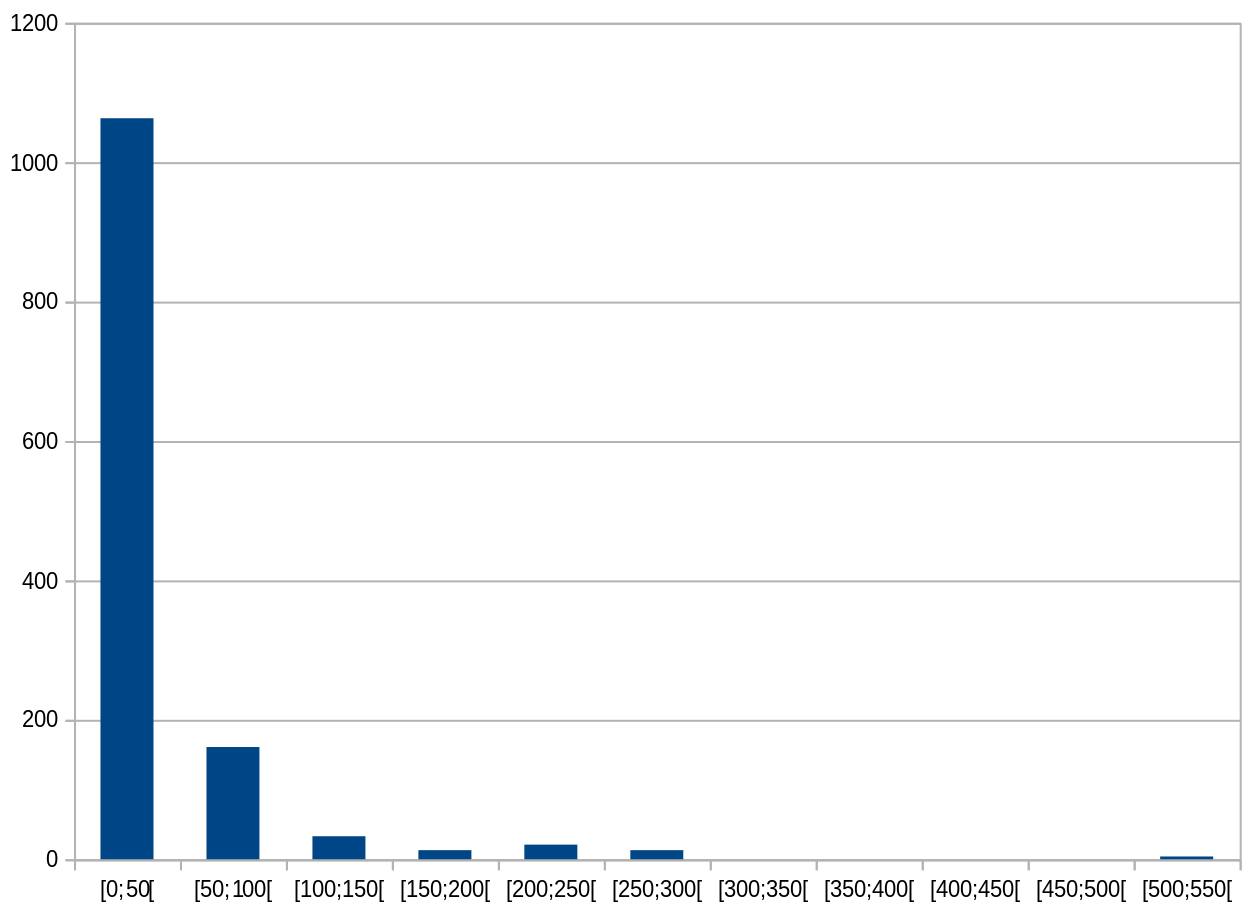
\includegraphics[width=8cm]{ressources/diagramme.png}
    \end{center}
\begin{aretenir}[]
L'icône \textbf{Insérer un diagramme} permet de construire des représentations graphiques dans LibreOffice.
\end{aretenir}
\end{frame}
\begin{frame}
    \frametitle{}

    \begin{activite}
    \begin{enumerate}
        \item Déterminer la moyenne des données du descripteur \emph{survie}. Quelle interprétation peut-on en donner ?
    \end{enumerate}
    \end{activite}

\end{frame}
\begin{frame}
    \frametitle{Avant de regarder la correction}
\begin{center}
    \centering
    \includegraphics[width=3cm]{/home/tof/Documents/Cozy/latex-include/stop.png}
    \end{center}
{\Large
    \begin{itemize}
        \item Prendre le temps de réfléchir,
        \item Analyser les messages d'erreur,
        \item Demander au professeur.
    \end{itemize}
}
\end{frame}
\begin{frame}[fragile]
    \frametitle{Correction}

    \begin{center}
        \begin{lstlisting}[language=Python , basicstyle=\small, xleftmargin=2em, xrightmargin=2em]
= MOYENNE(B2 : B1310)
\end{lstlisting}
        \captionof{code}{Survie}
        \label{age}
        \end{center}
    La moyenne de la colonne \emph{survie} est 0,38. Cela signifie que moins de la moitié des passagers ont survécu.

\end{frame}
\begin{frame}
    \frametitle{}
    Il n’y avait pas suffisamment de places dans les canots de sauvetage du Titanic pour tous les passagers et les membres de l’équipage (et certains canots sont partis à peine remplis). On souhaite examiner l’influence de la classe sociale des passagers sur l’obtention d’une place sur un canot de sauvetage.

    Pour calculer la fréquence de survie d'une classe, il faut, pour une classe donnée, calculer le rapport entre le nombre de survivants et le nombre total de passagers de cette classe.\\
    Pour calculer le nombre de survivants d'une classe, il peut être intéressant d'utiliser la fonction \textbf{\texttt{SOMME}}.
    

\end{frame}
\begin{frame}
    \frametitle{}

    \begin{activite}
        \begin{enumerate}
            \item Trier les données du descripteur \emph{classe} par ordre croissant à l’aide de l’autofiltre.
            \item Calculer la fréquence de survivants pour chaque classe.
        \end{enumerate}
        \end{activite}

\end{frame}
\begin{frame}
    \frametitle{Avant de regarder la correction}
\begin{center}
    \centering
    \includegraphics[width=3cm]{/home/tof/Documents/Cozy/latex-include/stop.png}
    \end{center}
{\Large
    \begin{itemize}
        \item Prendre le temps de réfléchir,
        \item Analyser les messages d'erreur,
        \item Demander au professeur.
    \end{itemize}
}
\end{frame}
\begin{frame}[fragile]
    \frametitle{Correction}

    \begin{center}
        \begin{lstlisting}[language=Python , basicstyle=\small, xleftmargin=2em, xrightmargin=2em]
= SOMME(B2:B324)/323
\end{lstlisting}
        \captionof{code}{Calcul pour la classe 1}
        \end{center} 
\begin{itemize}
    \item classe 1: 0,62
    \item classe 2: 0,43
    \item classe 3: 0,26
\end{itemize}
\end{frame}
\end{document}